\chapter{Przegląd literatury}
\label{cha:przegLiter}

%TODO OK ponieważ te opisy są dość obszerne proszę jednak dać to w osobne podrozdziały subsub (czy jak to wyjdzie)

\section{Zaawansowana binaryzacja i segmentacja + HOG SVM} %TT albo inaczej koledzy z poznania
W pracy \cite{kolzpoz} autorzy opracowali algorytm pozwalający na szybką i efektywną detekcję przechodniów w czasie rzeczywistym.
Termowizja pozwala na uzyskanie dobrego kontrastu między poszukiwanym przechodniem a otoczeniem.
Zaproponowany system jest dedykowany do pracy w nocy, kiedy kontrast między człowiekiem a otoczeniem pozwala na jednoznaczne ich rozróżnienie. %TODO OK między człowiekiem, a czym ?
Rozwiązanie bazuje na ulepszonym algorytmie progowania i segmentacji obrazu.

Pierwszym etapem jest wyodrębnienie obszarów zainteresowań (ROI).
Pozwala to na znaczne ograniczenie obszaru analizowanych fragmentów obrazu. %TODO OK rozmiaru analizowanych fragmentów obrazu (czy jakoś tak)
Obraz w odcieniach szarości zostaję poddany binaryzacji z użyciem dwóch progów: mniejszym i większym. Pozwala to na detekcję przechodniów w różnych rejonach obrazu o różnym kontraście.
Progi zmieniają się wraz z dynamiką obrazu wejściowego.
W obrazie termicznym człowieka często w okolicy bioder znajduje się chłodniejszy obszar, który jest poniżej progu binaryzacji, co skutkuje przerwę między dwoma połówkami człowieka. Aby połączyć je w jedną całość dodatkowo dla każdego obszaru wyłonionego podczas binaryzacji zostają wytypowane dodatkowe ROI, które obejmuje ten obszar wraz z innymi znajdującymi się nad lub pod. Przykładowy wynik segmentacji jest zaprezentowany na rysunku \ref{fig:S_IR}.

\begin{figure}
\centering
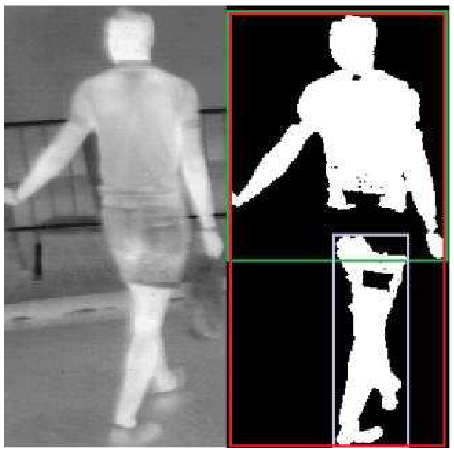
\includegraphics[width=0.4\linewidth]{images/S_IR}
\caption[Obraz IR po binaryzacji i segmentacji.]{Obraz IR po binaryzacji i segmentacji \cite{kolzpoz}}
\label{fig:S_IR}
\end{figure}
%TODO OK OK1. powt. dod, 2. niejasen
%TODO OK Proszę to kwestię dwóch progów lepiej opisać. Bo nie wiadomo jak co i po co jest robione.
%TODO OK to "tworząc" coś nie pasuje
%TODO OK to też jest niejasne.
%TT przepisałem ten akapit

Następnym krokiem jest filtracja wyników.
Ma ona na celu zredukowanie liczby obszarów przed końcową analizą.
Autorzy zastosowali filtrację opierającą się na proporcji obszaru zainteresowań.
Pozytywnie zakwalifikowane zostały jedynie obszary o odpowiednich proporcja wysokości do szerokości (1:1.3 do 1:4).
Z racji, że badany obraz pochodzi z kamery zamontowanej na stałe na samochodzie, autorzy wykorzystali filtrację perspektywiczną, która uwzględnia możliwą wysokość ROI w różnych fragmentach obrazu. %TODO OK tu jest coś nie tak...
Filtracja jednorodnych regionów pozwoliła na odrzucenie kandydatów będących częścią szerszych obiektów niemających nic wspólnego z przechodnimi. Obraz człowieka cechuje się dużą rozpiętością wartości temperatur. Obliczając odchylenie standardowe ROI w odcieniach szarości można wyeliminować obszary, które są poniżej progu określonego przez autorów. %TODO OK To jest niejasne...

Ostatnim krokiem algorytmu jest klasyfikacja wytypowanych kandydatów.
Autorzy wykorzystują histogram zorientowanych gradientów jako deskryptor, tworząc wektor 3780 cech, które są następnie klasyfikowane przez SVM.

W celu zbadania dokładności algorytmu został przeprowadzony test na zbiorze CVC-14, który zawiera obrazy nagrane kamerą FIR podczas nocnego przejazdu samochodem.
Testy wykazały, że metoda podwójnego progowania daje trzy razy lepsze rezultaty, niż przy wykorzystaniu pojedynczego progu. Wraz z zaproponowanymi technikami filtracji zaowocowało to bardzo efektywnym mechanizmem segmentacji. Ponad 95\% występujących przechodniów zostało poprawnie wytypowanych jako kandydaci do klasyfikacji.
%TODO ok no właśnie segmentacji czy klasyfikacji
Cała procedura detekcji przechodniów osiągnęła wysoki poziom wydajności na poziomie 33 klatek (o wymiarach 640x471 px) na sekundę przy wykorzystaniu pojedynczego rdzenia CPU. Dokładność detekcji wyniosła 37,3\% AMR
(ang. \textit{ Average Miss Rate }), która jest porównywalny do innych metod opartych o HOG+SVM.
%TODO A dla jakich parametrów strumienia wizyjnego.
%TT nie jest napisane wprost w artykule ale mam tą samą bazę i tam są 640 x 471.

\section{Stereotermowizja}
W pracy \cite{suard2006pedestrian} autorzy zaproponowali wykorzystanie dwóch kamer termowizyjnych tworząc system stereowizyjny. W obrazie termowizyjnym człowieka najcieplejszym obszarem jest zazwyczaj głowa. By wyodrębnić obszary zainteresowania, w~których potencjalnie znajdują się przechodnie, zgrupowano piksele o wartościach powyżej kilku różnych progów. Każdy z tych obszarów zostaje następnie uznany za głowę i stanowi górną część okna detekcyjnego. Wielkość okna jest estymowana na podstawie odległości źródła ciepła od kamer. Odległość jest ustalana na podstawie mapy dysparycji (ang. \textit{Disparity Map}). Do obliczani dysparycji okna, porównywana jest różnica między oryginalnym oknem a oknem przesuwnym w drugim obrazie. Na koniec każde okno zostaje przeskalowane do wielkości 64x128 i poddane klasyfikacji za pomocą liniowego SVM. %TODO OK znowu za mało szczegółów...
%TODO OK to raczej, z tego, że ZWYKLE głowa (stricte twarz) ew. dłonie są odsłoniete, wynika, że są widoczne jako najcieplejsze... bo tak ogólnie to chyba temperatura jest względnie równomiarna.

W pracy autorzy skupili się na optymalnym doborze parametrów deskryptora HOG. Wykorzystany zestaw danych zawierał 4400 obrazów: 2200 próbek z pieszymi oraz 2200 bez pieszych. Autorzy przeprowadzili po 10 procedur uczenia klasyfikatora dla każdej kombinacji wykorzystując różne zestawy danych do nauki i testów. W tabeli \ref{tab:parametryhog} zaprezentowane są wyniki tych testów. Badanie parametrów dla klasyfikacji SVM wykazało, że im większy zestaw uczący, tym lepszą można uzyskać skuteczność detekcji.

\begin{table}[!h]
\centering
\begin{threeparttable}
\caption{Parametry HoG.}
\label{tab:parametryhog}
\begin{tabularx}{1\textwidth}{|l|X|X|}

\hline Parametr & Zestaw do testów & Najlepszy wynik \\
\hline Rozmiar komórki & 4x4, 8x8, 16x16 & 8x8 \\
\hline Rozmiar bloku & 1x1, 2x2, 4x4 & 2x2 \\
\hline Nakładanie się komórek między blokami & 1,2 & 1 \\
\hline Schemat normalizacji bloków & brak, L1, L2 & L2 \\
\hline Liczba przedziałów histogramu & 4, 8, 16 & 8 \\
\hline Rodzaj histogramu & ważony, nie ważony & ważony \\
\hline

\end{tabularx}
\end{threeparttable}
\end{table}




%TODO Wnioskuję, że to liniowy SVM był - proszę to jawnie napisać.





%TODO Opis tego trzeciego algorytmu jest to poprawki !!! %TT  usunięty
% \section{Do wywalenia}
% Autorzy pracy \cite{nanda_2002} przedstawili metodę opartą o wzorzec probabilistyczny i klasyfikator Bayesa. 
% Obraz wejściowy zostaje zbinaryzowany z zadanym progiem. 
% Próg ten nie jest stały i zależy od wielu czynników. 
% %TODO a można konkretniej ? Np., że zostało to omóione poniżej
% Autorzy bazując na danych uczących stanowiących 1000 prostokątnych okien o rozmiarze 48x128 pikseli zawierających przechodnia średnią oraz odchylenie standardowe wartości dla pikseli należących do obrazu przechodnia \( \mu_1 \sigma_1 \) bądź tła \( \mu_2 \sigma_2 \) a następnie obliczyli próg binaryzacji za pomocą równia \eqref{eq:treshold_nanda}. %TODO OK odwołania do równiań poprzez eqref. , te symbole jakoś w tekście nie są w nawiasie
% %TODO To zadnie to jest jakiś "potworek" proszę poprawić.
% 
% \begin{equation} \label{eq:treshold_nanda}
% threshold = \frac{\sigma_1 \sigma_2}{ \sigma_1 + \sigma_2} \ln\left ( \frac{\sigma_1}{\sigma_2} \right ) + \frac{\sigma_1\mu_1 + \sigma_2\mu_1}{\sigma_1+\sigma_2}\end{equation}
% 
% Aby uzyskać wzorzec prawdopodobieństwa, zbiór testowy został zbinaryzowany z uprzednio wyliczonym progiem. 
% Następnie zostało obliczone prawdopodobieństwo przynależności piksela do przechodnia we wzorcu. %TODO To jest ciut niejasne.
% Mając już wzorzec, został obliczony combinedpropability ze wzoru \eqref{eq:combo_nanda} dla 1000 okien zawierających i nie zawierających człowieka oraz wyciągnięta średnia i odchylenie standardowe dla nich. 
% 
% %TODO To com.... to trzeba na coś zamienić !!!
% 
% Dało to podstawę do obliczenia progu dla wartości combinedpropability z wzoru \eqref{eq:treshold_nanda}. 
% %TODO to jest jakieś niejasne.
% 
% \begin{equation} \label{eq:combo_nanda} combinedprobability(i,j)=\sum_{x=1}^{48}\sum_{y=1}^{128}(th(x,y)*p(x,y)+(1-th(x,y))*(1-p(x,y)))\end{equation}
% \noindent
% gdzie \(th(x,y)\) to okno wokół piksela \((i,j)\), a \(p(x,y)\) to wzorzec prawdopodobieństwa wystąpienia pieszego.
% 
% Badana klatka obrazu jest badana poprzez okno przesuwne tworząc mapę prawdopodobieństwa. %TODO badana klatka jest badana ? 
% Wartości które przekroczą próg wskazują, że w danym oknie znajduje się człowiek. 
% 
% %TODO ale jakie wartości ? 
% Autorzy zbadali algorytm na 6 sekwencjach filmowych i uzyskali wynik między 75\%-90\% wykrycia przy jednym fałszywym wykryciu na ramkę. %TODO chyba średnio jednym...

%TODO Tutaj omówienie tych algorytmów z Poznania

\section{Podejście sprzętowo-programowe. Stereowizja dla robotów }

W pracy \cite{honegger2014real} autorzy wykorzystali układ FPGA oraz CPU małej mocy do skonstruowania systemu wizyjnego dla robotów.
System analizował obraz stereoskopowy z dwóch kamer wizyjnych tworząc mapę głębi.
\begin{figure}[h]
\centering
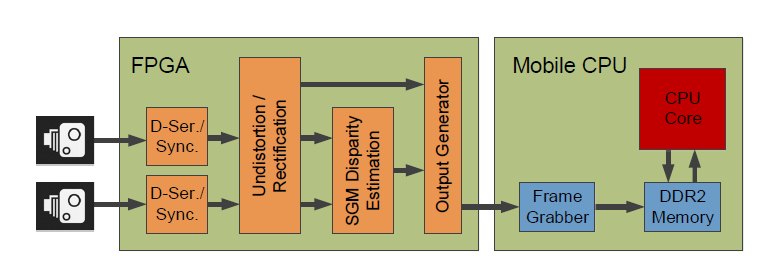
\includegraphics[width=1\textwidth]{images/honegger2014real_Fig1}
\caption{Schemat systemu wizyjnego zaproponowanego w pracy\cite{honegger2014real}.}
\label{fig:honegger2014real_Fig1}
\end{figure}
%TODO OK wizyjnych, czy termo
Obie kamery zostały bezpośrednio podpięte do układu FPGA za pomocą interfejsu LVDS (ang. \textit{Low-Voltage Differental Signal} – niskonapięciowy sygnał różnicowy), w którym obrazy były następnie przetwarzane.

%TODO OK proszę zwrócić uwagę na czas -> były (bo wcześniej wykorzystali) ogólnie takie badania opisuje się w czasie przeszłym.

Schemat systemu jest przedstawiony na rysunku \ref{fig:honegger2014real_Fig1}. W pierwszej kolejności obrazy z kamer są synchronizowane z wykorzystaniem bufora opóźniającego jedną linię danych.
Przychodzące, zsynchronizowane piksele są zapisywane do bufora. Korekcja zniekształceń soczewkowych oraz rektyfikacja zostały połączone w jedną operację. Po obliczaniu współrzędnych piksela uwzględniającym korektę, jego wartość jest pobrana z właściwej lokalizacji w buforze wejściowym. Kolejnym krokiem było obliczanie dysparycji. W tym celu kontekst piksela z lewego obrazu jest porównywany z okolicznymi kontekstami pikseli w prawym obrazie. Kandydat jest wyłaniany na podstawie lokalnej funkcji kosztu i stałych globalnych bazujących na algorytmie SGM (ang. \textit{Semi-Global Matching}).

Następnie dwa oryginalne obrazy oraz obliczona mapa głębi są przesyłane do CPU za pomocą specjalnej magistrali.
%TODO OK może magistrali
Moduł \textit{frame grabbera} przechwytywał ten obraz i wykorzystując DMA (ang. \textit{Direct Memeory Acces}) zapisywał do pamięci systemu.
%TODO OKno to jest niejasne... tzn. ta pierwsza część zdania.
System pracował w rozdzielczości 752x480 pikseli i 60 klatkach na sekundę.
Całość, włącznie z kamerami, układem FPGA, CPU oraz konwerterami napięcia pobierał mniej niż 5W mocy.
Całkowita latencja podana przez autorów rozwiązania wynosi około 2ms.

%TODO ale to coś jeszcze robiło ? Bo rozumiem, że FPGA liczyło stereo (pytanie jak) i do CPU trafiały te obrazy. Ale coś więcej się działo ?
%TT niestety nie, po prostu szybko liczyło obraz stereo z wykorzystaniem fpga

\section{Podejście sprzętowo-programowe. System wspomagania kierowcy}
W pracy \cite{piao2016real} autorzy wykorzystali układ SoC (ang. System on Chip) do detekcji pieszych dla zaawansowanego systemu wspomagania kierowcy (ADAS ang. \textit{Advanced Driver Assistance System}).
Głównym wyzwaniem było opracowanie systemu, która działa w czasie rzeczywistym, ma mały pobór mocy oraz niski koszt wykonania.
%TODO OK raczej systemu/rozwiązania (szczególnie koszt wykonania dla algorytmu jest dyskusyjny)
Najbardziej skuteczne algorytmy wymagają znacznych zasobów obliczeniowych. %TODO topowych -> słowo potoczne i do zmiany
Autorzy dokonali zatem relaksacji problemu poprzez zastosowanie prostszego deskryptora, jakim jest LBP oraz klasyfikatora SVM.
Po każdej stronie pojazdu została zamontowana inteligentną kamerę o szerokim, 180$^\circ$ horyzontalnym kącie widzenia, by jak najlepiej monitorować przestrzeń wokół niego.
%TODO wyeliminiować powt. autorzy
W kamerach została przeprowadzona wstępna obróbka obrazu (rektyfikacja i skalowanie).
%TODO rektyfikacja ? czyli to był system stetero ?
%Nie był to system stereo ale w artykule wyraźnie piszą o rektyfikacji, choć podejrzewam że chodziło im o korekcje soczewkową
Przetworzony obraz z kamer był transmitowany do \textit{''Fusion-Box''}, gdzie odbywała się generacja kandydatów, klasyfikacja, weryfikacja oraz śledzenie.
Wyniki były przesyłane do wbudowanego komputera PC.
Rozwiązanie nie zostało jeszcze w pełni zaimplementowane, ale pierwsze testy dawały obiecujące rezultaty.

\section{Wzorzec probabilistyczny}
\label{sec:xiao_2015}
W pracy \cite{xiao_2015} autorzy wykorzystali układ FPGA i naiwny klasyfikator Bayesa do detekcji przechodniów w obrazie termowizyjnym. Klasyfikator zakłada, że wszystkie predykatory są niezależne od siebie, co znacznie upraszcza obliczenia. Za pomocą tego klasyfikatora można określić przynależność obrazu w badanym oknie do jednej z dwóch klas: zawierającego przechodnia albo który nie zawiera (czyli tła). W tym przypadku predyktorami są poszczególne piksele. Dla każdego piksela w oknie określa się prawdopodobieństwo jego przynależności do danej klasy. Klasyfikacja sprowadza się do zależności \eqref{eq:bayes_china}.
%TODO OK do za ??? poza tym to jest coś niejasne}
%TT opis poprawiony

\begin{equation} \label{eq:bayes_china}
\sum_{x,y} \ln p(w_{x,y}|P) > \sum_{x,y} \ln p(w_{x,y}|\bar{P})
\end{equation}

\noindent gdzie \( p(w_{x,y}|P) \) to prawdopodobieństwo, że piksel $w_{x,y}$ przynależy do obrazu człowieka
\( p(w_i|\bar{P}) \) przynależy do tła.
%TODO no ale co to jest i, bo czegoś tu nie rozumiem....
Jeżeli nierówność jest prawdziwa wtedy okno zostaje sklasyfikowane jako zawierające przechodnia.
Obrazy wykorzystane w systemie są binarne, co oznacza, że \( p(w_{x,y}|P) \) przyjmuje dwie wartości, w zależności czy jest to piksel czarny czy biały. Można w ten sposób stworzyć macierz rozkładu prawdopodobieństwa (PDM ang. \textit{probability distribution matrix})która określa prawdopodobieństwo wystąpienia białego piksela w oknie (prawdopodobieństwo wystąpienia czarnego jest \(1- p(w_{x,y}|P) \)). Inną nazwą tej macierzy jest wzorzec probabilistyczny.
Autorzy utworzyli PDM na podstawie 60 pozytywnych próbek.

W celu usprawnienia obliczeń w układzie FPGA macierz została przeskalowana na wartości całkowitoliczbowe w zakresie od 1 do 127.
Następnie obliczono logarytm o podstawie dwa z uzyskanego wzorca i jej odwrotności (poprzez odjęcie od 128 wartości macierzy pozytywnej) i pomnożono przez 32. %TODO OK powt. następne
Utworzono tak dwie macierze: LPDW i LPDB dla białych i czarnych pikseli. (ang. \textit{Logarithmic Probability Matrix} – logarytmiczna macierz prawdopodobieństwa).
Przyjęto, że prawdopodobieństwo przynależności piksela do tła jest stałe i wynosi 50\%, co daje wartość 192 po uprzednich przekształceniach.
Ostatecznie klasyfikacji dokonuje się z wzoru:
%TODO OK raczej klasyfikacji dokonuje się...

\begin{equation}\label{equ:Lp}
L_{p} = \sum_{x=1}^{j}\sum_{y=1}^{k}(th(x,y)*LPMW(x,y)+(1-th(x,y))*LPMB(x,y))
\end{equation}
\begin{equation}\label{equ:Lb}
L_{b} = j*k*192
\end{equation}
\begin{equation} \label{equ:ispedistant}
IsPedestrian = \left\{ \begin{array}{ll}
1 & \textrm{gdy $L_{p} \geq L_{b} + K$}\\
0 & \textrm{gdy $L_{p}<L_{b} + K$}
\end{array} \right.
\end{equation}

\noindent gdzie $j$ i $k$ stanowią wysokość i szerokość okna przesuwnego. Wartości $L_p$ i $L_b$ odnoszą się do sum prawdopodobieństw przynależności białego/czarnego piksela do obrazu człowieka. $K$~jest parametrem którym określono minimalną wartość dla której klasyfikator daje poprawne pozytywne wyniki.

W omawianej pracy autorzy opracowali wzorce dla 3 różnych wielkości okna: 10x15, 8x12 i 6x9 pikseli. Do stworzenia wykorzystali jedynie górne połówki obrazu termicznego ludzkiej sylwetki, co miało na celu bardziej niezawodnego wzorca wobec różnych postur przechodniów.
\section{Praca Inżynierska}
Praca inżynierska \cite{kankaing} oraz artykuł na jej podstawie\cite{kanka2016fpga}, której kontynuacją jest mniejsza praca, rozwinęła koncepcję zaproponowaną w sekcji \ref{sec:xiao_2015}. Zastosowano 4 wzorce o wymiarach 48x120, 32x80, 24x60,19x48. Wzorzec został podzielony na 4 części: górną, dolną, prawą lewą. Następnie, podobnie jak w DPM, układ tych 4 części decydował o jego klasyfikacji. Każda część tworzyła maskę wielkości całego okna. Jeżeli co najmniej 3 takie maski pokrywały się obszar ten był klasyfikowany pozytywnie. Pozwoliło to na znaczną poprawę działania algorytmu, co pokazuje wykres ROC przedstawiony na rysunku \ref{fig:analiza_wykres}.

\begin{figure}
\centering
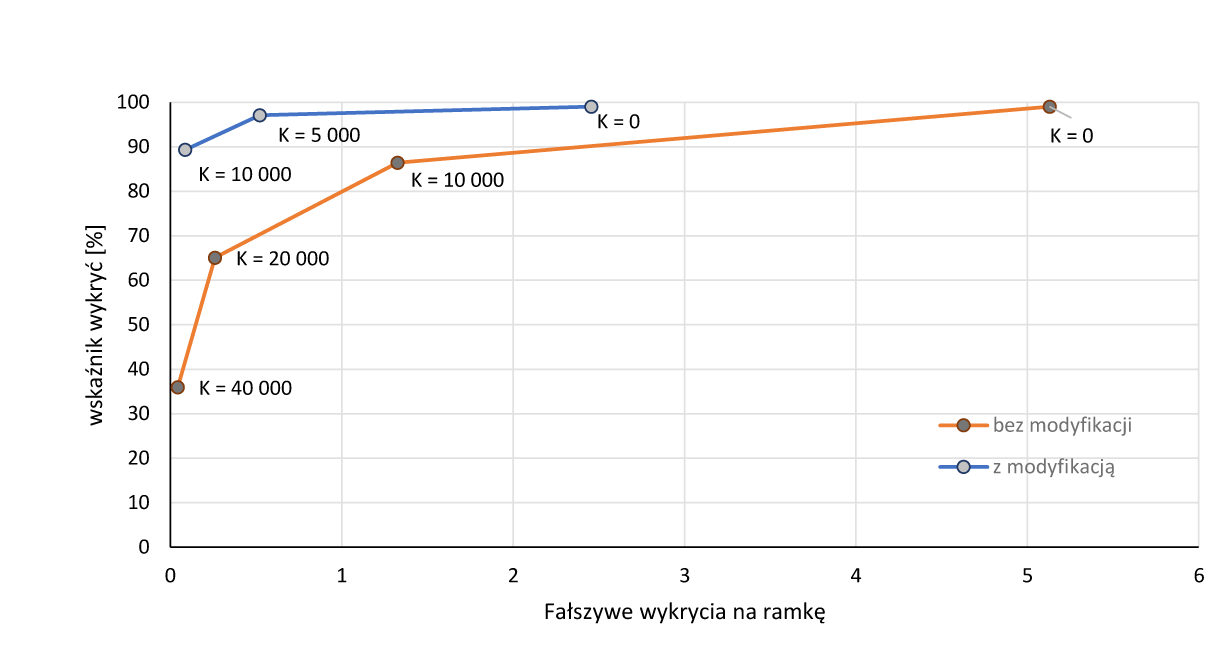
\includegraphics[width=0.8\linewidth]{images/Analiza_wykres}
\caption[Wykres REC]{Wyniki symulacji przy różnych wartościach parametru K.\cite{kankaing}}
\label{fig:analiza_wykres}
\end{figure}

Poprawiło to również detekcję w różnych skalach. Poprzednio \textit{muliscale} osiągnięto dzięki zastosowaniu kilku wzorców. Pojedynczy wzorzec zapewniał detekcję w pewnym zakresie wysokoci przechodniów. Im dalej odbiegiał od swojej nominalnej wysokości, tym bardziej należało zmniejszyć parametr $K$ by w pojedynczym oknie było możliwe wykrycie mniejszych i większych sylwetek. Powodowało to również zwiększenie ilości fałszywych detekcji. Po wprowadzeniu modyfikacja każda część ma możliwość deformacji, co w dynamiczny sposób pozwala na zmianę wysokości wzorca.

\begin{figure}
\centering
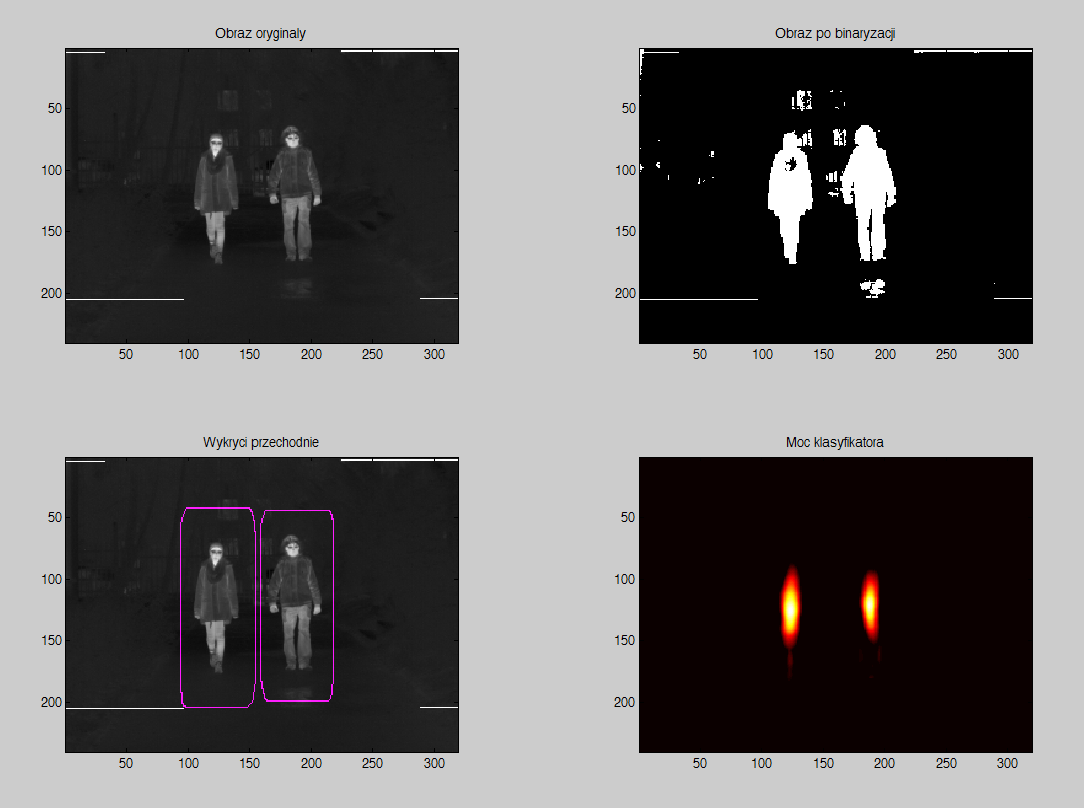
\includegraphics[width=0.8\linewidth]{images/sim_window.png}
\caption[Proces detekcji wzorcem probabilistycznym.]{Proces detekcji wzorcem probabilistycznym. \cite{kankaing}}
\label{fig:sim_window}
\end{figure}

Dodatkową ciekawą właściwość można zauważyć na rysunku \ref{fig:sim_window} przedstawiającym implementację systemu w programie Malab. Okno przedstawiające ''moc klasyfikacji'' ($L_p - (L_b + K)$ ) wyraźnie widać dwa maksima lokalne wskazujące dokładną pozycję przechodniów. Ta właściwość została wykorzystana w niniejszej pracy w celu ustalenia ROI.
%TODO OK ogólnie ta metoda (z p. inż. też jest jakoś nie do końca fajnie opisana) - proszę to dopracować.
%TODO OK dalej - proszę "pochwalić" się artykułem na ten temat - przecież powstał



